\documentclass[../../main.tex]{subfiles}
 
\begin{document}

Radio-frequency (RF) phased arrays have applications in radar telemetry, telecommunications, ground-penetrating radar, scientific instrumentation, and remote sensing \cite{Vieregg_2016,AVVA201746,arnold_2020,PhysRevD.105.122006,10.3390/s21186091,10.1016/j.jappgeo.2022.104876,phased_array_book}.  In the one-dimensional case, $N$ three-dimensional RF antennas are arranged in a line with fixed spacing.  In the two-dimensional case, $N \times M$ three-dimensional antenna elements are arranged in a two-dimensional grid with fixed spacing in both dimensions.  The signal to noise ratio (SNR) of received signals in arrays of dimension $N$ is boosted by a factor of $\approx \sqrt{N}$, because the $N$ signals are combined coherently while thermal noise adds like $\sqrt{N}$.  The SNR boost is critical for certain kinds of scientific observations.  For example, systems created at the Center for Remote Sensing and Integrated Systems (CReSIS) are flown in polar regions to perform radar sounding of ice sheets for the purposes of geophysics and climate science \cite{arnold_2020}.  Reflected signals carry information about the ice depth, temperature, and internal structure of the ice.  The radio echoes have small SNR values that require phased arrays.  \\ \vspace{2.5mm}

Traditionally, RF phased arrays are designed with commerical computational electromagnetism (CEM) software.  Radio antennas and phased arrays have \textit{radiation patterns} that define directions of maximum transmission power and received sensitivity.  Radiation patterns have a main lobe in which most of the radiation is concentrated, and the angular width of the main lobe is called the beam width.  Other parameters like S-parameters quantify the efficiency of the systems.  CEM packages like XFDTD and HFSS are used to model these properties as a function of frequency \cite{remcom,ansys}.  The XFDTD package, for example, relies on the finite difference time domain (FDTD) method. The FDTD approach is a CEM technique in which spacetime and Maxwell’s equations are broken into discrete form.  HFSS uses a similar approach in the Fourier domain, the Finite Element Method (FEM).  Depending on the software license and version, the current price of these products ranges between \$5,000 and \$40,000 USD.  These costs are prohibitive for HSI undergraduate institutions like Whittier College.  Removing this financial barrier to entry would enable diverse researchers to gain important skills in the field of RF design. \\ \vspace{2.5mm}

Another drawback of commercial CEM software is the lack of access to the source code, which impedes the incorporation of modern machine learning packages.  Phased array properties are determined by the shape of the RF elements and the grid properties of the array, and the parameter space is driven by the complex variety of RF element shapes.  When combined with open-source CEM software, modern machine learning algorithms can locate optimal solutions within the parameter space.  The authors of \cite{10.3390/electronics8121506} review a number of open-source CEM packages, and conclude that there are viable open-source options for simple RF antenna shapes.  For our proposed work, the open-source CEM software must be able to handle the growing complexity of RF antenna designs.  One interesting choice is the MIT Electromagnetic Equation Propagation (MEEP) package \cite{10.1016/j.cpc.2009.11.008}.  Though MEEP was designed for $\mu$m wavelengths in photonics applications, we have shown that the scale-invariance of Maxwell's equations allows MEEP users to translate designs to wavelengths at the cm-scale.  We have also shown that MEEP can drive the RF phased-array design loop, and that 3D printer schematics can be extracted from this process \cite{electronics10040415,meepcon2022,10.1016/j.cpc.2009.11.008}.  This research represents an opportunity for diverse undergraduates to gain experience applying machine learning tools to the design of practical systems.  \\ \vspace{2.5mm}

Recent advances in materials research have led to the creation of 3D printer filament that has conductivity in RF bands.  Funded through an NSF Translational Impact (TI) award (1721644), Multi3D LLC. has produced filament with a resistivity of just $10^{-2} \Omega$ cm: the Electrifi filament.  Several antenna designs have already been produced \cite{8786183,10.1049/iet-map.2017.0104}.  These examples include horn antennas with gain factors of 15 dB at 5.8 GHz, and microstrip patch antennas with gains of 1-2 dB at 2.5 GHz.  The results match expectations from HFSS models, exhibiting no major differences with antennas made using perfect conductors.  There are, however, virtually no examples of 3D printed RF phased arrays in the [0.1 - 1] GHz bandwidth.  This bandwidth is the most relevant for the aforementioned applications in particle astrophysics and geophysics.  Further, whole new designs can be discovered that improve on designs like the horn and patch antennas by merging machine learning packages with MEEP.  In Sec. \ref{sec:cem}, we review progress already made at Whittier College.  In Sec. \ref{sec:askaryan}, we show how this work enhances the field of UHE-$\nu$ observations.  In Sec. \ref{sec:cresis}, we show how this work enhances the field of radio echo sounding of ice sheets and ice shelves.  In Sec. \ref{sec:int}, we articulate our vision for the integration of this research into our STEM curriculum at Whittier College.  In Sec. \ref{sec:conc_im}, we make the case that the overall intellectual merits of the proposed activities are sound.

\section{Computational Electromagnetism and Additive Manufacturing}
\label{sec:cem}

In Summer 2020, we received a Faculty Fellowship from the Office of Naval Research (ONR) to study and design phased arrays in the [0.1 - 5] GHz bandwidth.  This bandwidth is relevant for projects like IceCube Gen2 (radio), and Whittier College is a member institution of the IceCube Gen2 collaboration.  With our background in NSF-funded projects like the Antarctic Ross Ice Shelf Antenna Neutrino Array (ARIANNA), the Askaryan Radio Array (ARA), and NASA-funded projects like the Antarctic Impulsive Transient Antenna (ANITA), we were qualified to teach our ONR colleagues about phased array applications.  Our goal was to design a phased array system to be integrated as a transmitter in an anechoic chamber.  The anechoic chamber will serve as a testing facility for active radar systems.  We began by giving lectures on the electromagnetism of phased arrays and scientific and engineering applications.  The audience included engineers and programmers that work in acquisition and development for the Naval Surface Warfare Center (NSWC), Corona Division (NSWC Corona).  Our design flow is depicted in Fig. \ref{fig:design}.  To minimize costs and increase access to Whittier College students, we decided to investigate open-source CEM options for the design. \\ \vspace{2.5mm}

\begin{figure}
\centering
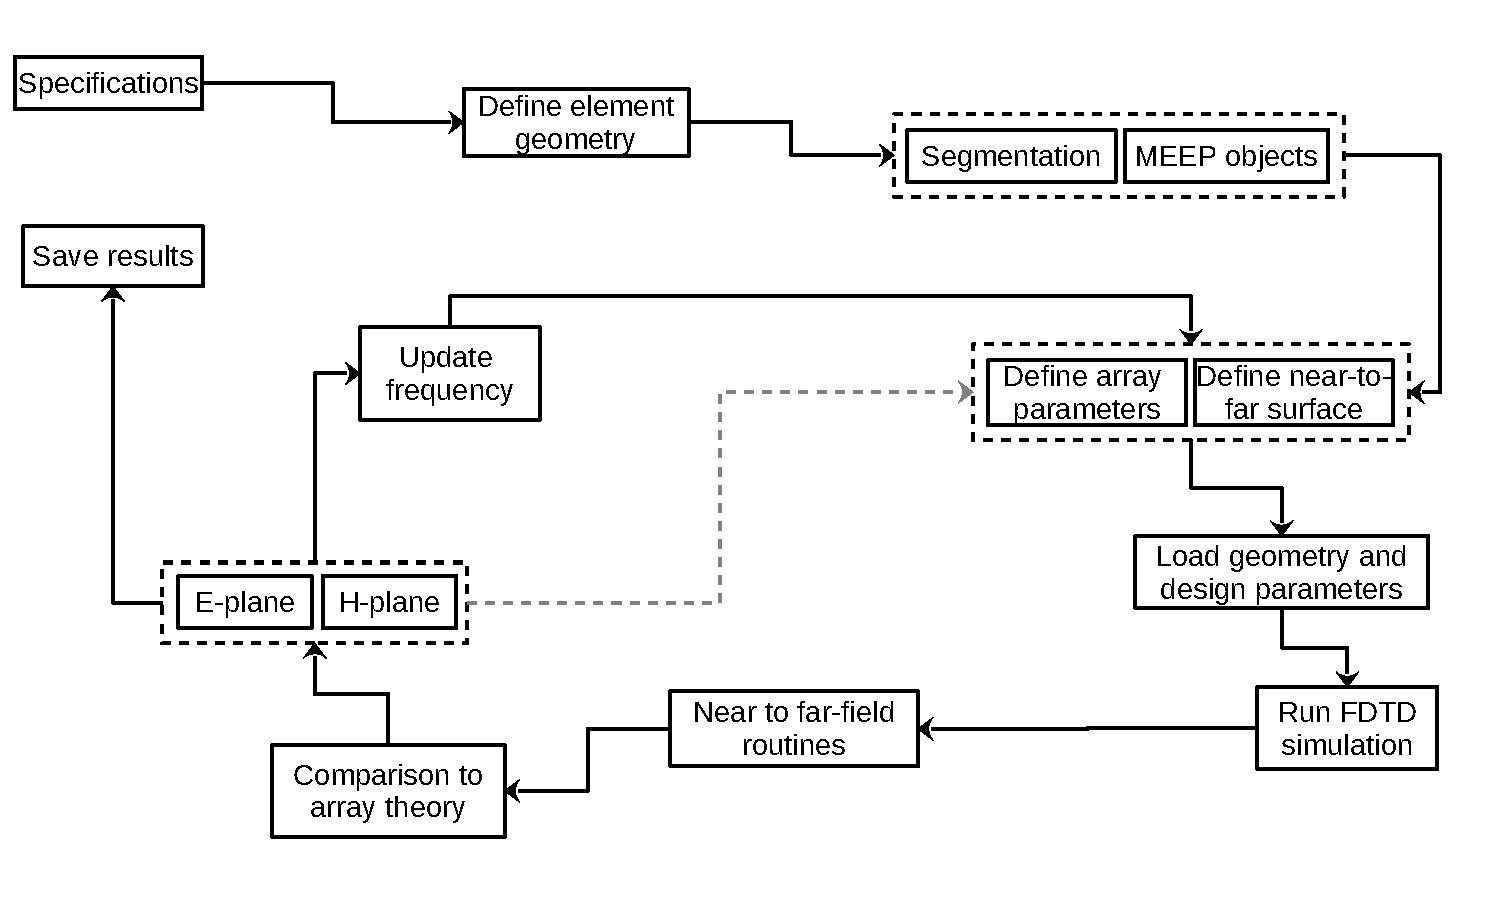
\includegraphics[width=0.85\textwidth]{diagram3.pdf}
\caption{\label{fig:design}  Our design process for RF phased arrays from \cite{electronics10040415}, adapted from Fig. 1 of the review \cite{10.3390/electronics8121506}.}
\end{figure}

We encountered the aforementioned review article in the open-access journal \textit{Electronics} that indicated there are open-source CEM tools that can be adapted to phased array analysis.  Our design flow in Fig. \ref{fig:design} is adapted from Fig. 1 of the review to include specific tasks required for phased arrays, and algorithms for the computation of far-field radiation patterns.  MEEP was noted by the authors in the review as the most advanced among open-source FDTD programs, but they did not benchmark it against HFSS or XFDTD due to the ``steep'' learning curve.  As part of the ONR Summer Faculty Fellowship, we ascended the learning curve and adapted MEEP to RF systems.  The key insight was that MEEP takes advantage of the \textit{scale invariance} of Maxwell's Equations.  The simplest way to understand this is to understand how MEEP uses relative units when discretizing Maxwell's equations for Python code. \\ \vspace{2.5mm}

Like other FDTD CEM methods, MEEP uses a Yee lattice to discretize Maxwell's equations \cite{10.1109/tap.1966.1138693}.  When the speed of light is set to unity ($c = 1$), distance and time units are set to be the same.  Frequency and wavelength units are the inverse of each other.  But distance and wavelength can take \textit{any} unit of length in the Yee lattice.  Most MEEP users interpret this unit of length to be 1 $\mu$m because the applications are for photonics.  For example, a \textit{relative} frequency (unit-less) of 0.5 corresponds to a \textit{relative} wavelength of 2.  When interpreted as 2 $\mu$m, the frequency is 150 THz in real units that correspond to optical bandwidth.  If we choose to interpret the \textit{relative} wavelength as 2 cm, the real frequency is 15 GHz.  A \textit{relative} frequency of 0.05 corresponds to the RF frequency 1.5 GHz.  Assuming design components have sufficient conductivity at RF frequencies, we have re-purposed MEEP as an RF simulator.  \\ \vspace{2.5mm}

\begin{figure}
\centering
%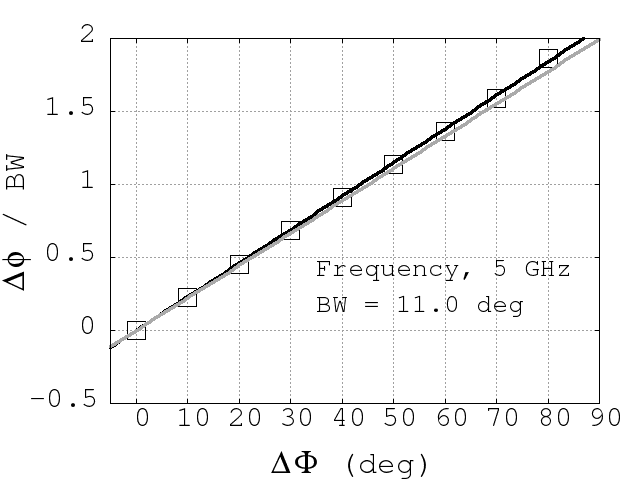
\includegraphics[width=0.35\textwidth]{figures/Oct30_plot2.png}
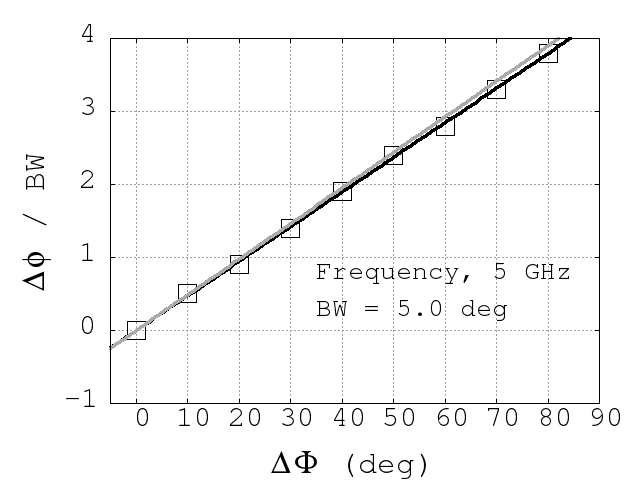
\includegraphics[width=0.33\textwidth]{figures/Oct30_plot1.png}
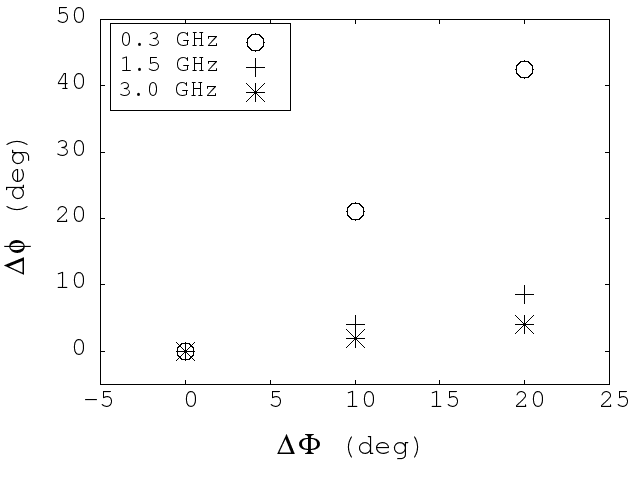
\includegraphics[width=0.33\textwidth]{figures/Aug11_plot2.png}
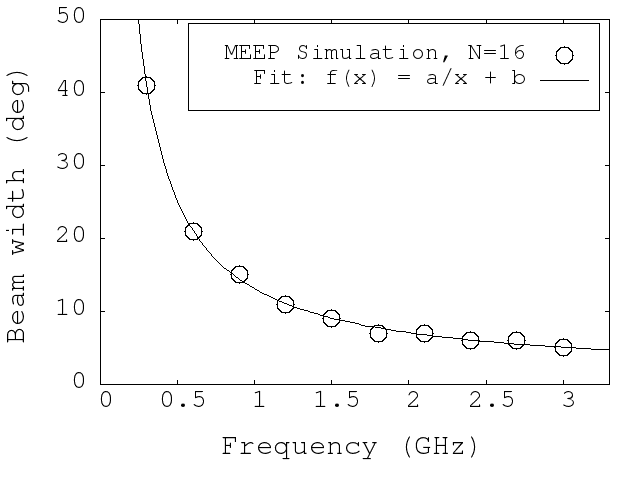
\includegraphics[width=0.33\textwidth]{figures/Aug11_plot1.png}
\caption{\label{fig:pa_1} (Left) The beam angle $\Delta \phi$ divided by the beam width $BW$ for the $N = 16$ one-dimensional Yagi array versus $\Delta \Phi$, the phase shift per element. The gray line represents theoretical expectation, and the black line is a linear fit to the data.  (Middle) $\Delta \phi$ versus $\Delta \Phi$ for the $N=16$ version of the one-dimensional horn array, for several frequencies.  (Right) The dependence of the beam width on frequency for the one-dimensional $N=16$ horn array.  The black line is a functional fit to the data $f(x) = a/x + b$ with $a=12.0\pm 0.1$ degree GHz, and $b=1.1\pm 0.2$ degrees.}
\end{figure}

By Fall 2020, we were producing CEM models using MEEP that matched expected phased array properties.  For a one-dimensional array with $N$ elements, there is a linear relationship between the radiated plane-wave direction $\Delta \phi$, and the phase shift per element $\Delta \Phi$.  The coefficient of the relationship is determined by the ratio of real wavelength to element spacing.  Figure \ref{fig:pa_1} contains results for our first phased array models in which the elements were Yagi-Uda style antennas and horn antennas.  The linear relationship is evident in the data.  The radiated signal direction $\Delta \phi$ is divided by the beam width (BW) in Fig. \ref{fig:pa_1} (left), and is left in degrees in Fig. \ref{fig:pa_1} (middle).  A beam width of a radiation pattern is the angular width of the main lobe, outside of which the radiated power has decreased by 3 dB.  In Fig. \ref{fig:pa_1} (left), the $N=16$ Yagi array can steer a 5 GHz plane wave up to four beam widths to the right or left of the forward direction.  Yagi-Uda style antennas are designed for a single frequency.  In Fig. \ref{fig:pa_1} (middle), results are shown for an $N=16$ array of horn antennas.  Since horn antennas are broadband radiators, the linear relationship is shown for 0.3, 1.5, and 3.0 GHz.  The beam width is inversely related to frequency, so $\Delta \phi$ was left in degrees.  In Fig. \ref{fig:pa_1} (right), the inverse relationship is shown. \\ \vspace{2.5mm}

We can also produce phased array radiation patterns with MEEP that match theoretical expectations.  The radiation pattern of a one-dimensional array of $N$ radiating point sources can be derived using first principles \cite{electronics10040415}.  The \textit{pattern multiplication theorem} states that the radiation pattern of a one-dimensional phased array of $N$ identical elements will be that of a row of $N$ point sources, multiplied by the radiation pattern of the individual element.  In Fig. \ref{fig:1dhornresults2} (left and middle), the radiated field of a $N=16$ horn array is shown in the E-plane (x-y plane).  The radiation pattern is shown in \ref{fig:1dhornresults2} (right).  The main lobe is steered 9 degrees above the x-axis, matching the theoretical expectation.  The blue curve in the polar plot represents the CEM radiation pattern from MEEP, while the red curve is the theoretical expectation from a row of $N$ point sources.  The row of point sources is symmetric, creating a back lobe at $\Delta \phi = 171$ degrees.  The horn array has no back lobe because the individual horns suppress backward radiation, as expected from the pattern multiplication theorem.  We also showed that two-dimensional arrays of Yagi-Uda and horn antennas matched theoretical expectations exactly.  Our revelation that the photonics code MEEP could used to design phased arrays design earned the final article Top 10 honors for December 2020 to May 2021 from the editors of \textit{Electronics}. \\ \vspace{2.5mm}

\begin{figure}
\centering
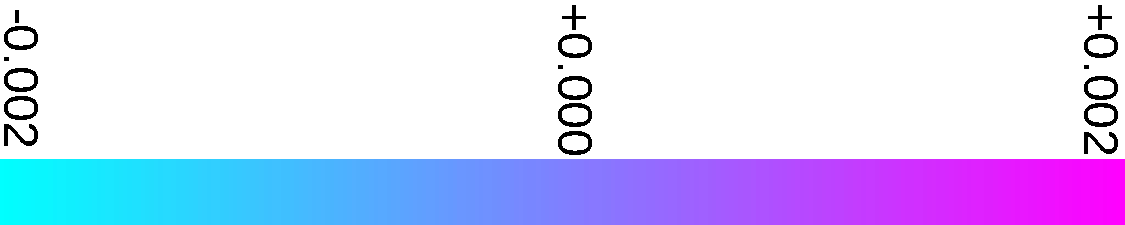
\includegraphics[width=5.625cm,angle=90]{figures/fields/colorbar.pdf}
%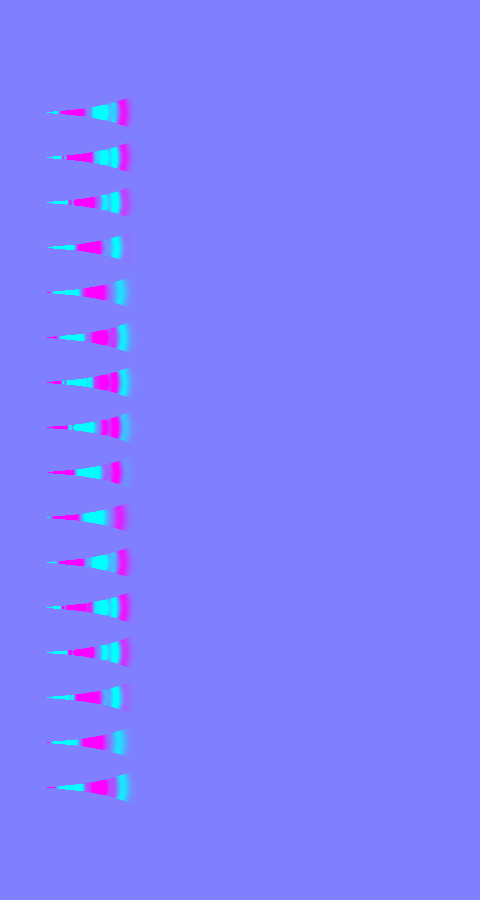
\includegraphics[width=3cm]{figures/fields/ey_phase_horn_t15.png}
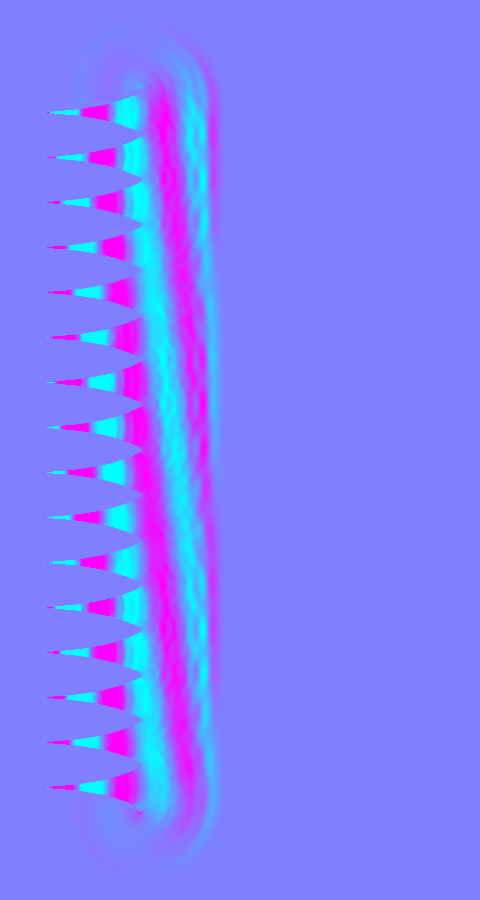
\includegraphics[width=3cm]{figures/fields/ey_phase_horn_t30.png}
%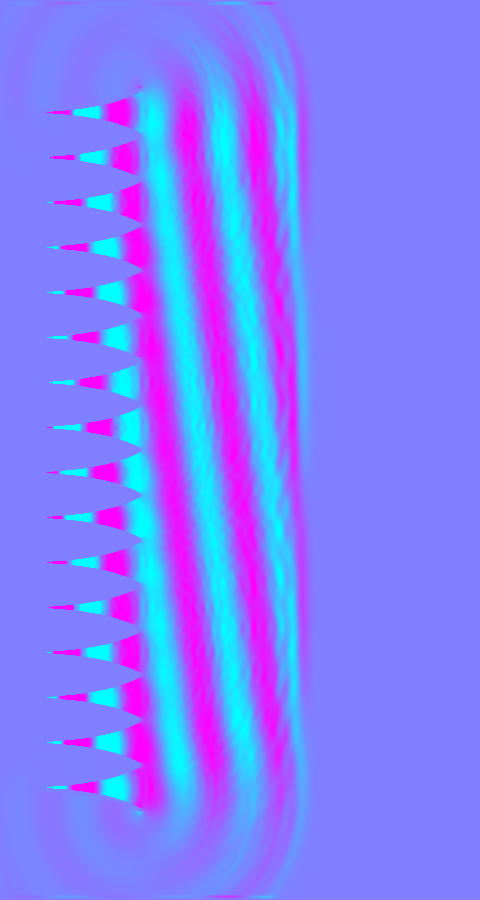
\includegraphics[width=3cm]{figures/fields/ey_phase_horn_t45.png}
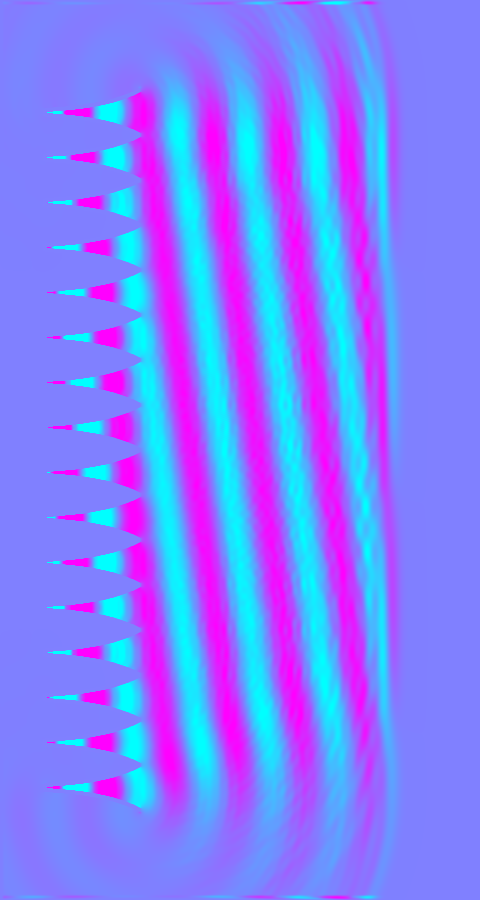
\includegraphics[width=3cm]{figures/fields/ey_phase_horn_t60.png}
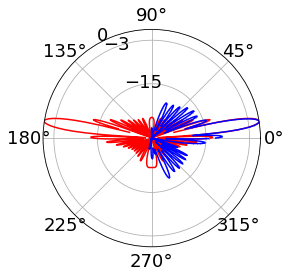
\includegraphics[width=6cm]{figures/fields/rad_patt_field.png}
\caption{\label{fig:1dhornresults2} (Left) The $N = 16$ one-dimensional horn array, radiating a linearly polarized electric field $\vec{E}(x,y,t)$ (y-component shown, in arbitrary units) at $t = 1$ ns into the simulation run, and (middle) at $t = 2$ ns into the run.  The 2D area is $80 \times 150$ cm$^2$.  The frequency is 2.5 GHz, and the beam angle is $\Delta \phi = 9$ degrees from broadside (x-direction). (Right) The normalized radiated power in dB versus $\Delta \phi$.  The blue curve represents the results from MEEP, and the red curve is the theoretical expectation from $N$ point sources.}
\end{figure}

It is important to note that our undergraduate physics, computer science, and engineering curriculum is greatly enhanced by researching applications of CEM.  One straightforward example is to incorporate CEM tools like MEEP into lower and upper division electromagnetism and Python3 courses.  Our 3-2 Engineering Program students, Physics majors, and Integrated Computer Science (ICS) majors all stand to benefit from learning to use Python to perform computational physics.  Our current curriculum does not yet include CEM in lower or upper-division electromagnetism courses, nor is it included in computational physics.  Integrating results from this research into course management systems, via MEEP Jupyter notebooks, is a straightforward way to enhance STEM education for our diverse undergraduates.  Showcasing the 3D printed RF systems should engage their curiosity by providing a real-world application of course concepts.  Finally, given the diverse demographics of our students, enriching their educational experience with real-world applications serves to diversify the STEM workforce.  We propose to develop project-based learning (PBL) modules that incorporate RF design, machine-learning, and additive manufacturing for our Whittier College STEM students.  \\ \vspace{2.5mm}

\begin{figure}
\centering
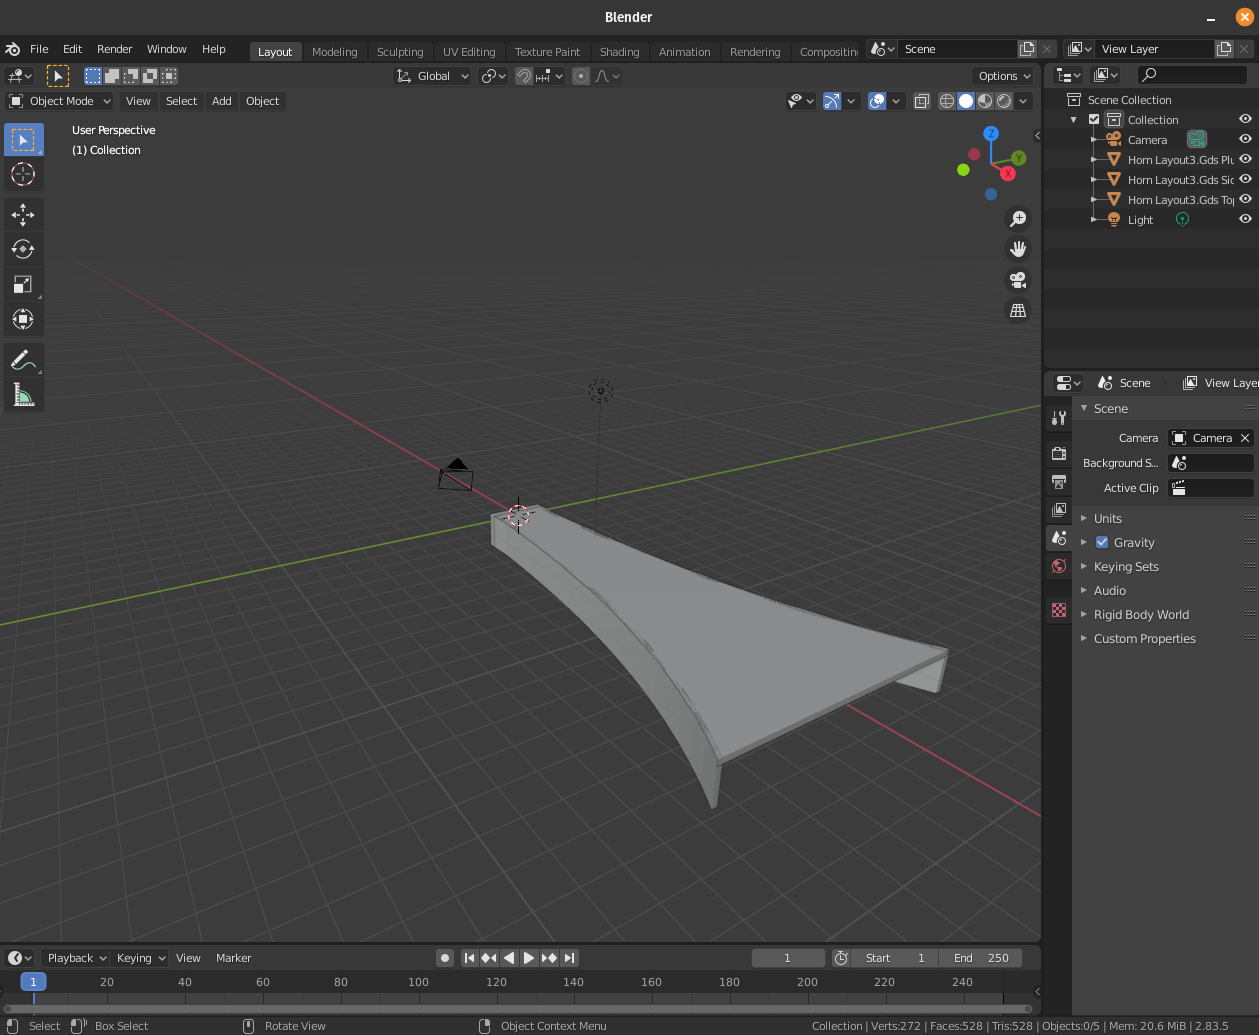
\includegraphics[width=0.35\textwidth]{figures/blender_example.png}
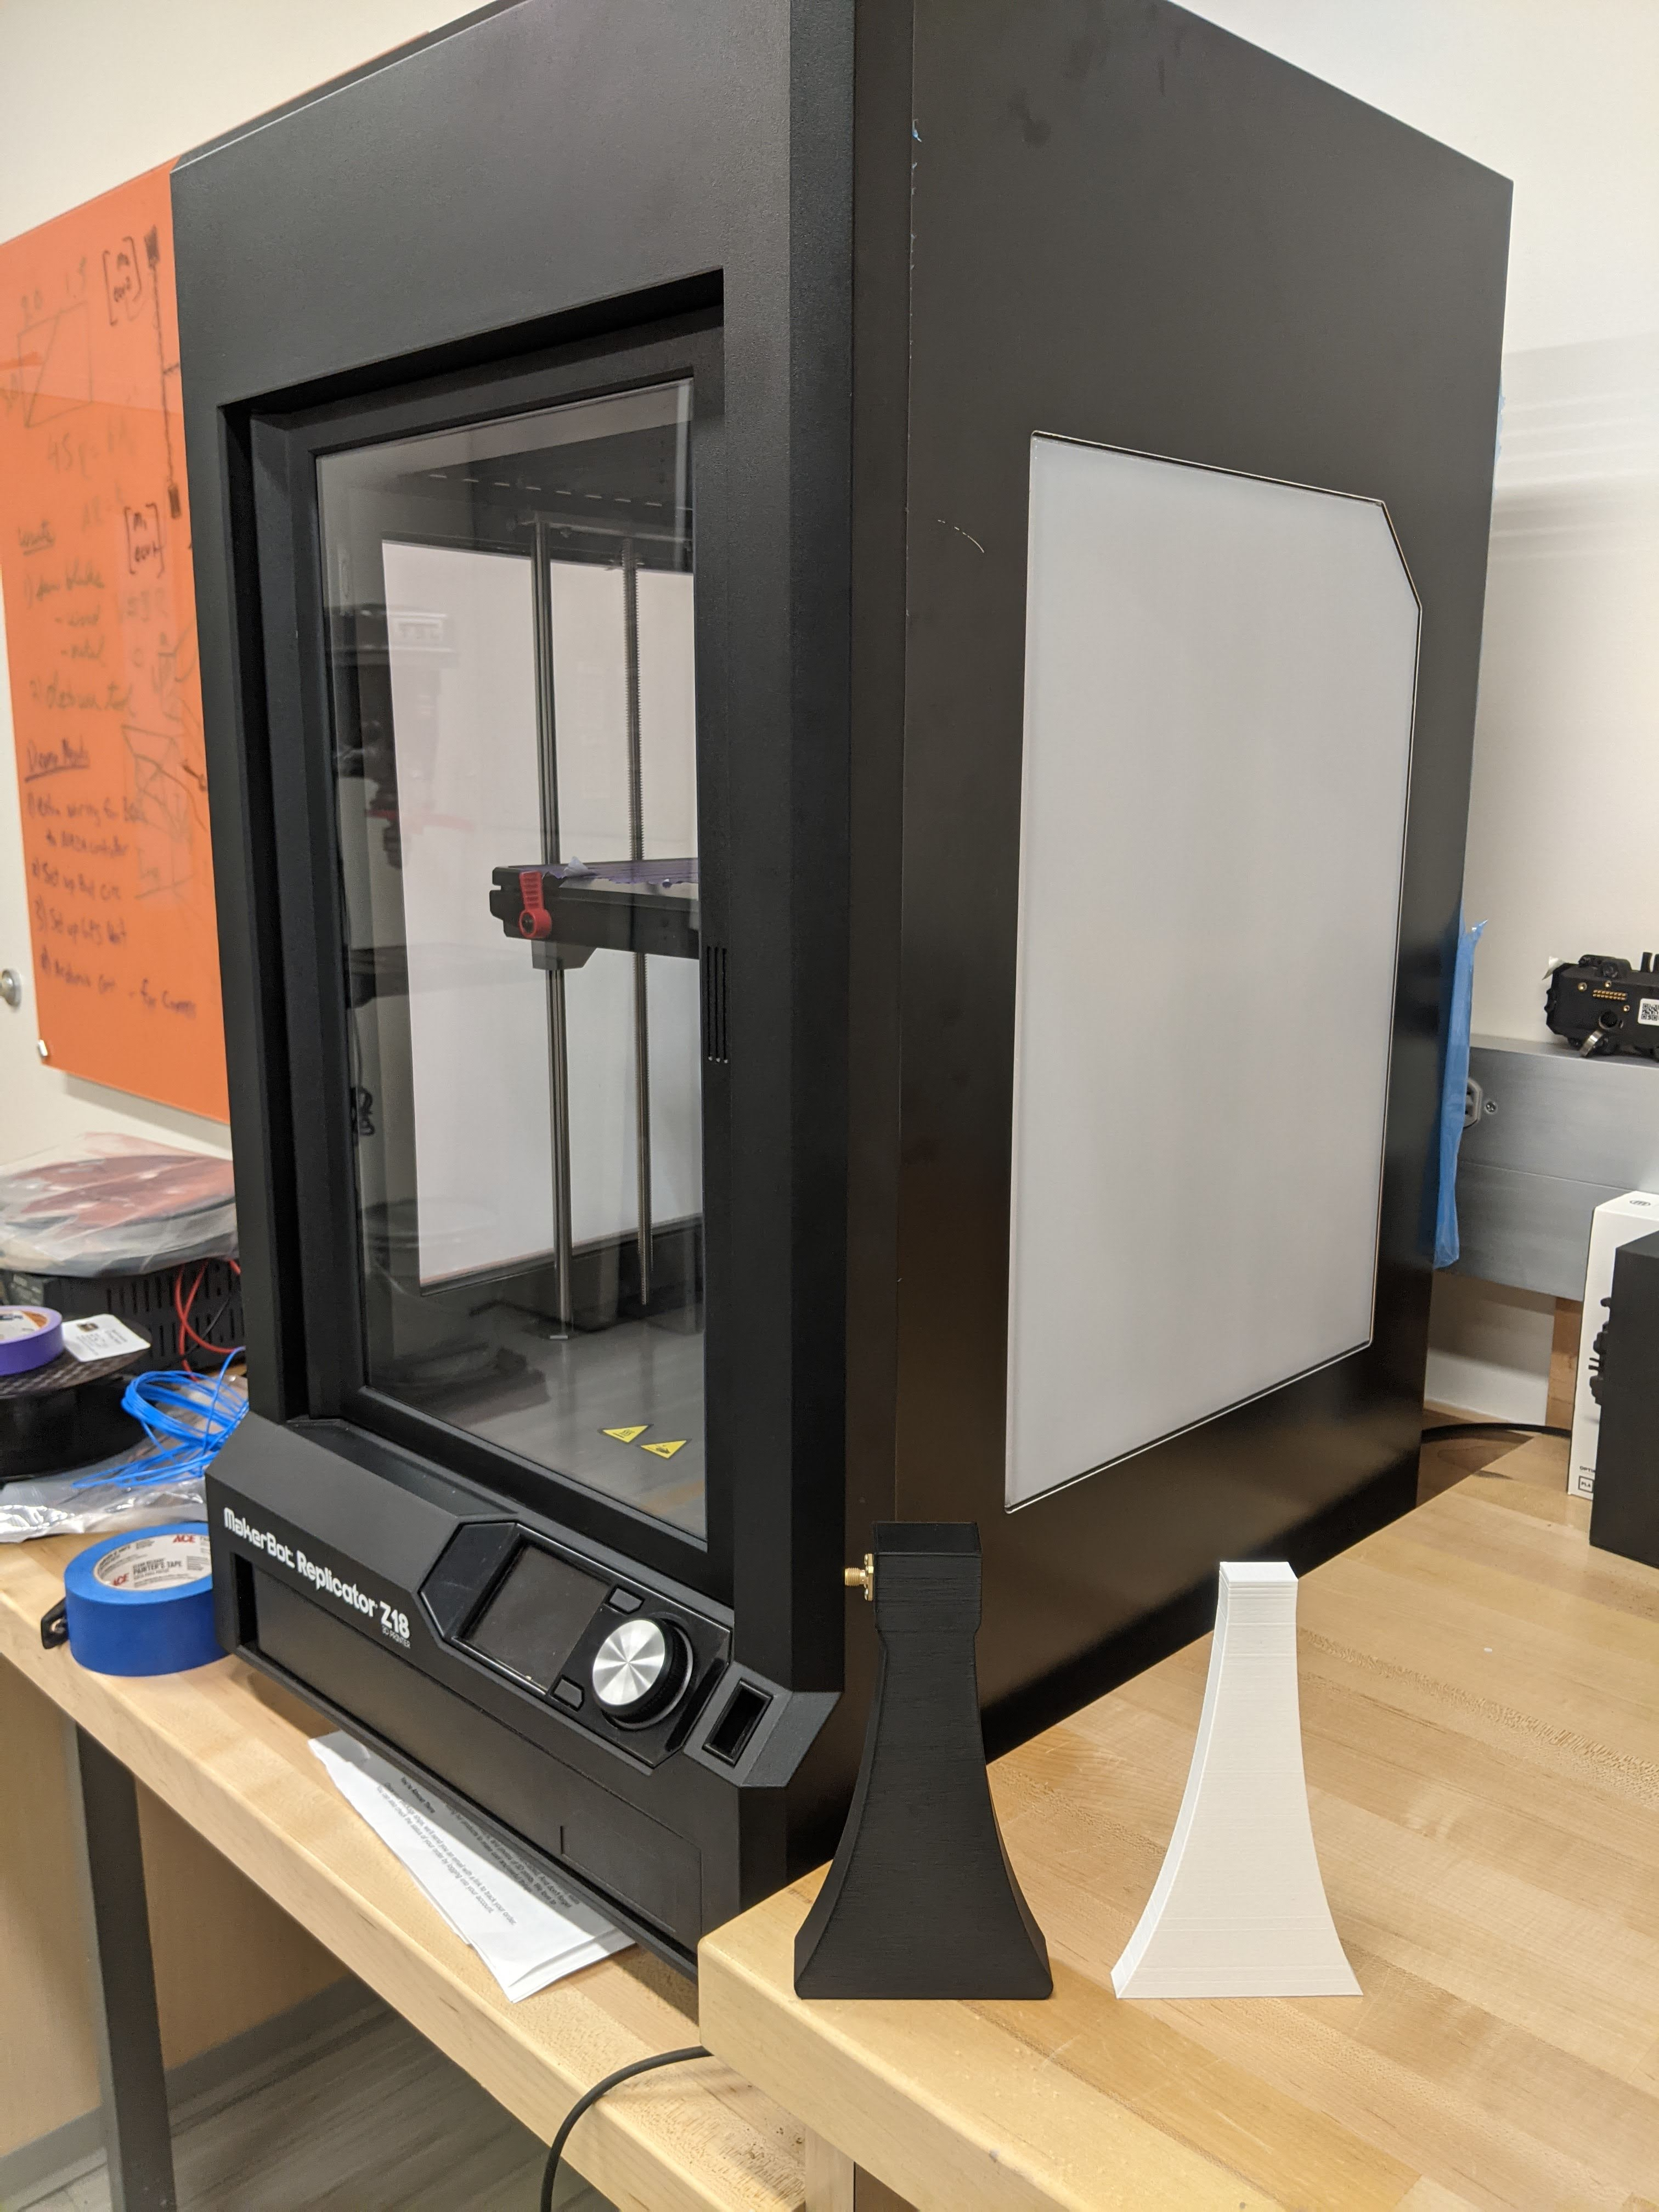
\includegraphics[width=0.3\textwidth]{figures/3dprinter.jpg}
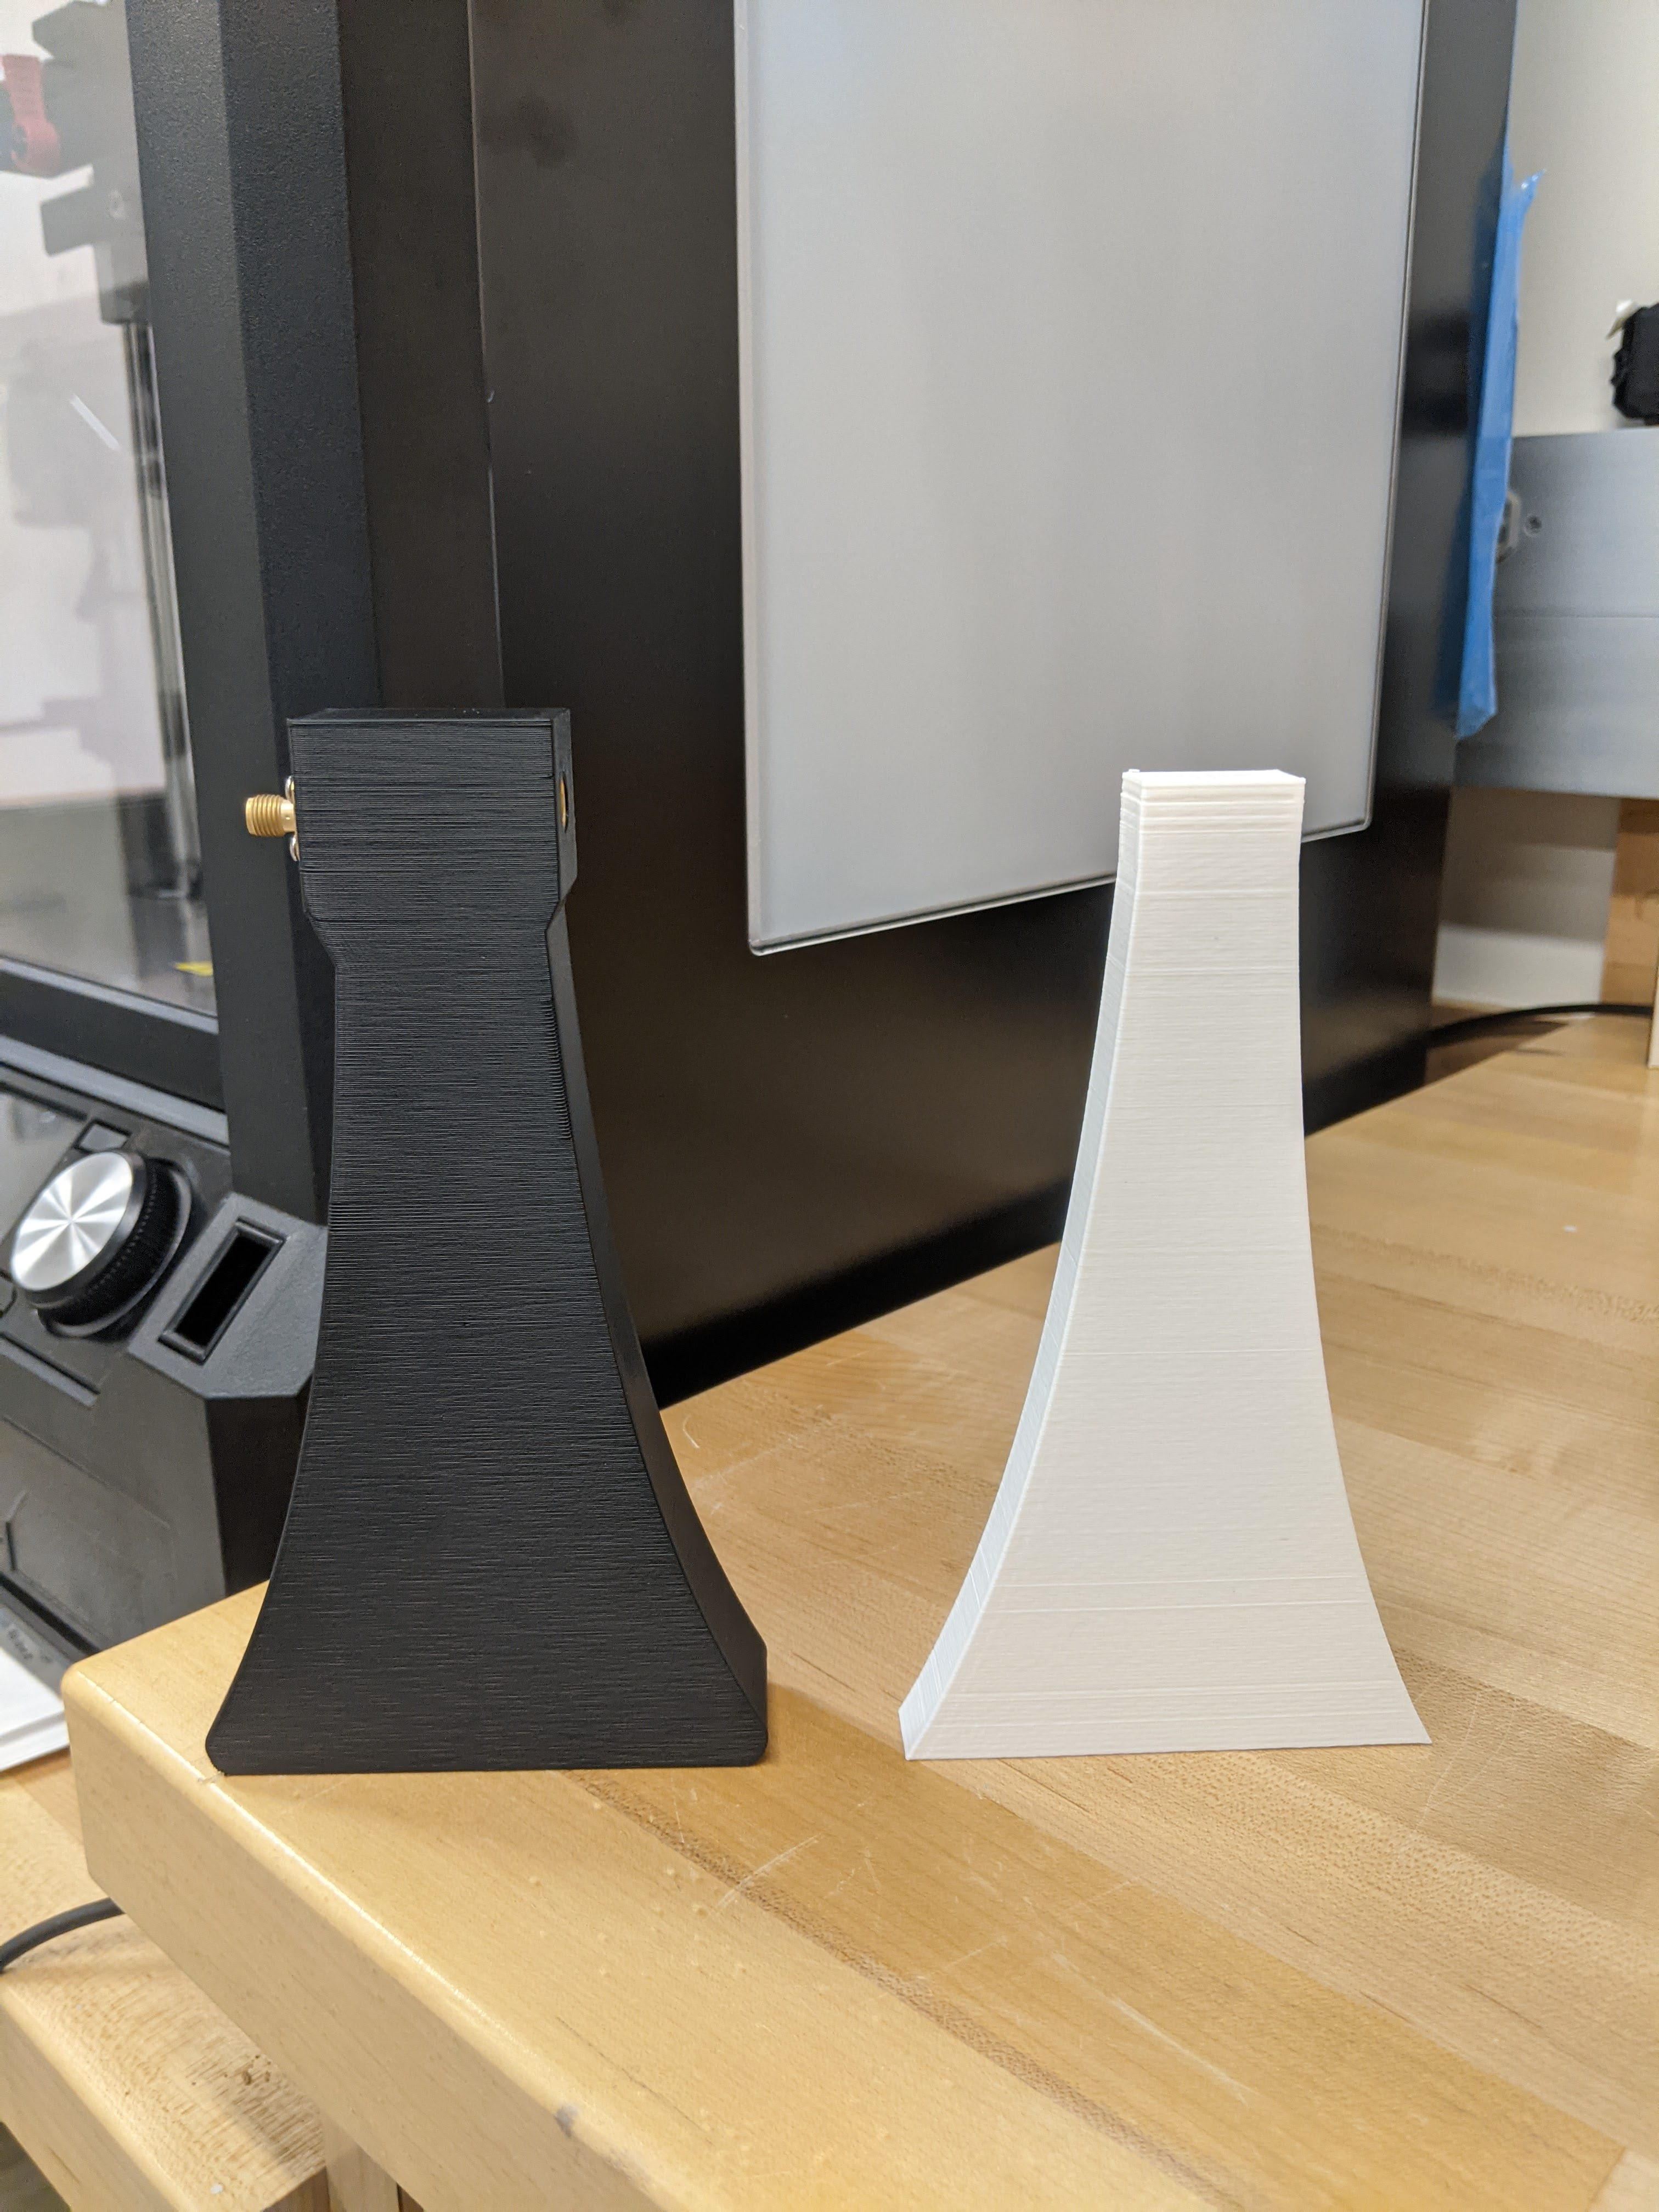
\includegraphics[width=0.3\textwidth]{figures/3dprinter_2.jpg}
\caption{\label{fig:3d_print} (Left) Blender/STL files extracted from MEEP code.  (Middle) MakerBot 3D printer, with PLA horn model (white), and  proto-pasta with SMA connector (black). (Right) Close-up of horns.}
\end{figure}

\begin{figure}[hb]
\centering
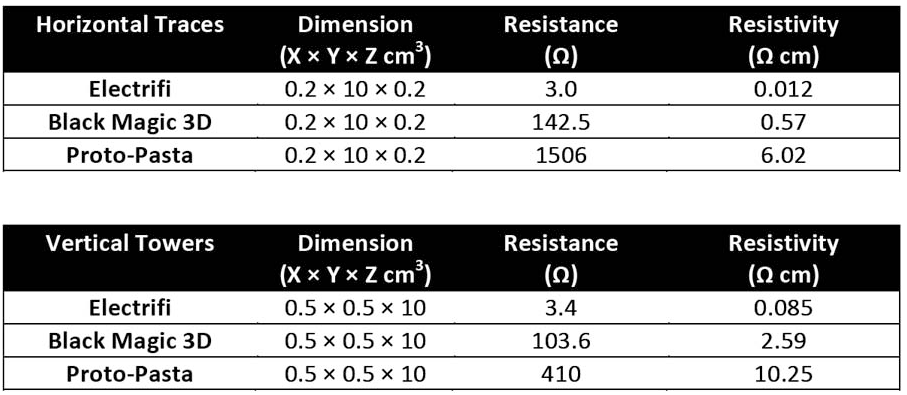
\includegraphics[width=0.65\textwidth]{figures/multi3dllc.png}
\caption{\label{fig:3d_print2} Resistivity results published by Multi3D LLC that compare the proto-pasta product with the new Electrifi conductive filament (\url{https://www.multi3dllc.com/faqs/}).}
\end{figure}

In Summer 2021, we again received a Faculty Fellowship from the ONR to continue this work.  We focused on creating realistic 3D models of horn antennas that could be printed with 3D printers.  Working with undergraduate researchers, we learned to create designs that can be expressed as Python3 functions and converted to a GDSII CAD file.  GDSII files can be imported into MEEP, and converted to STL files for use with a 3D printer.  Our CEM codes are therefore using the precise shape that we intend to print.  We acquired NinjaTek proto-pasta 3D printer filament, advertised as conductive.  We printed a horn with in-built SMA connecter for RF cables (Fig. \ref{fig:3d_print}). The proto-pasta result had the right shape, but a measured resistance too large for an RF antenna.  Multi3D LLC, the manufacturer of the Electrifi filament, has now provided resistivity results that compare proto-pasta with Electrifi (Fig. \ref{fig:3d_print2}).  The Electrifi filament will improve resistivity by two orders of magnitude.  We seek to print Electrifi-based antennas, and to measure the radiation pattern and S-parameters. \\ \vspace{2.5mm}

In Summer 2022, we received a final ONR Faculty Fellowship that focused on GPS M-code and modernization.  Alongside this work, we continued to refine the open-source RF horns.  This included computing radiation patterns and S-parameters for the full 3D horns stored in CAD files.  In Fig. \ref{fig:3d_cad} (a), the main lobes are designed to point to 0 degrees (x-direction) for the E-plane (x-y plane), and 90 degrees for the H-plane (x-z plane).  The E-plane is the plane containing the linearly polarized radiation vector, and the H-plane is orthogonal to the E-plane.  In Fig. \ref{fig:3d_cad}, the (voltage standing wave ratio) VSWR is shown.  The VSWR is a common figure of merit for RF antennas, related to the S11 scattering parameter.  The VSWR approaches 1 for an efficiently radiating antenna.  The radiation patterns match expectations for horn antennas (see Fig. 19 of \cite{8786183}).  The VSWR results demonstrate efficient radiation in the bandwidth [0.5 - 6] GHz.  We presented our progress at the annual MeepCon 2022 at the Massachusetts Institute of Technology (MIT) \cite{meepcon2022}.  We learned the extent to which MEEP can be integrated with Python3-based machine learning tools \cite{meepcon2022_2}, and how eager MEEP developers are to collaborate in the RF regime.  Extending MEEP to RF users widens the user base of MEEP, which has traditionally focused on photonics applications.

\begin{figure}
\centering
\begin{subfigure}{0.65\textwidth}
    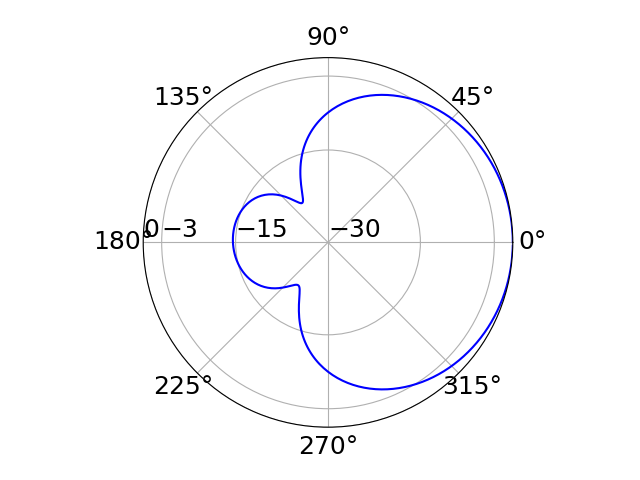
\includegraphics[width=0.49\textwidth]{figures/3DHorn_CAD_0_5GHz_E_plane.png}
	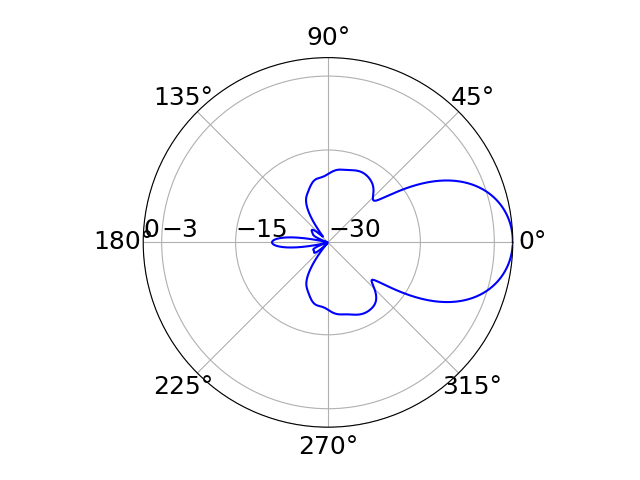
\includegraphics[width=0.49\textwidth]{figures/3DHorn_CAD_5GHz_E_plane.png} \\
	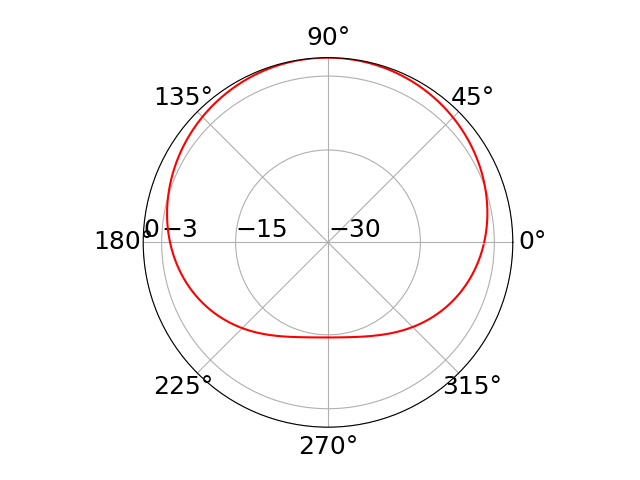
\includegraphics[width=0.49\textwidth]{figures/3DHorn_CAD_0_5GHz_H_plane.png}
	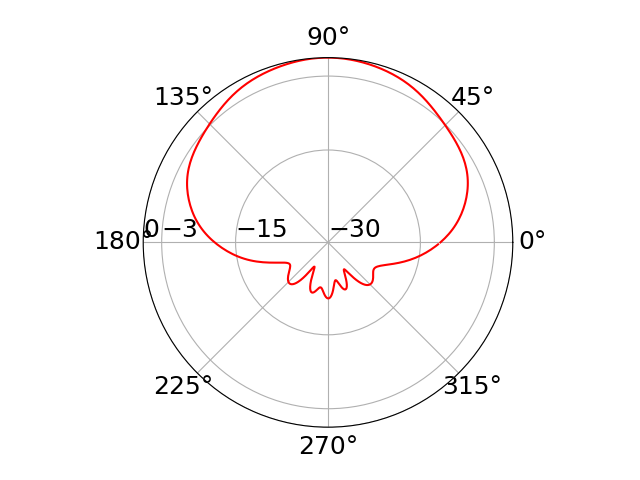
\includegraphics[width=0.49\textwidth]{figures/3DHorn_CAD_5GHz_H_plane.png}
    \caption{Radiation pattern results using GDSII/CAD for (top left) E-plane at 0.5 GHz, (top right) E-plane at 5.0 GHz, (bottom left) H-plane at 0.5 GHz, (bottom right) H-plane at 5.0 GHz.  See text for details.}
\end{subfigure}
\hfill
\begin{subfigure}{0.3\textwidth}
    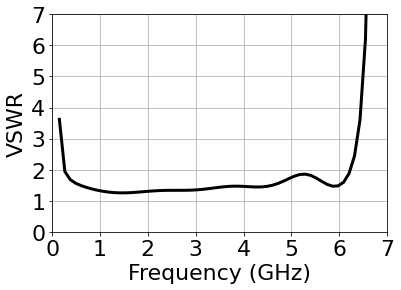
\includegraphics[width=0.99\textwidth]{figures/vswr.png}
	\caption{The VSWR figure of merit versus frequency in GHz for the RF horn.}
\end{subfigure}
\caption{Results for RF horn design, using the open-source design process open to 3D printing.}
\label{fig:3d_cad}
\end{figure}

\subsection{RF Laboratory Capability}

We have founded an Educational Partnership Agreement (EPA) between NSWC Corona and Whittier College.  As part of the EPA, NSWC Corona has the ability to transfer technology 

...

According to ONR protocols, I become eligible for Senior Faculty Fellowships once I have been awarded an SFRP Fellowship three times.  I am eligible to apply in Summer 2023 after a mandatory one-year cooling period.  I have included all funding I have received from the ONR, and all student fellowships that I have received up to the present in Tab. \ref{tab:funds}.  I have included all equipment NSWC Corona has donated to Whittier College in Tab. \ref{tab:equip}.  These items were at first on loan to us, but are now being converted to donations.  There are further HPC resources in preparation to be donated to us, pending approval by senior personnel at the lab.  Equipment such as the items in Tab. \ref{tab:equip} are typically donated to colleges and universities when their project life-cylce is complete at the Navy lab and are no longer necessary.  In Sec. \ref{sec:epa} below, I articulate a vision for the use of these instruments in Whittier College engineering projects.

\begin{table}[hb]
\centering
\begin{tabular}{c c c c}
Student/Professor & Grant Opportunity & Amount & Dates \\ \hline
Jordan C. Hanson & ONR Summer Faculty Fellow & \$16.5k & Summer 2022 \\
Raymond Hartig & Ondrasik-Groce Fellowship & \$5k & Summer 2022 \\
Jordan C. Hanson & ONR Summer Faculty Fellow & \$16.5k & Summer 2021 \\
Adam Wildanger & Fletcher Jones Fellowship & \$5k & Summer 2021 \\
Jordan C. Hanson & ONR Summer Faculty Fellow & \$16.5k & Summer 2020 \\
Raymond Hartig & Fletcher Jones Fellowship & \$5k & Summer 2020 \\
John Paul G\'{o}mez-Reed & Ondrasik-Groce Fellowship & \$7.5k & Summer-Fall 2019 \\
John Paul G\'{o}mez-Reed & Keck Fellowship & \$5k & Summer 2018 \\
Cassady Smith & Keck Fellowship & \$5k & Summer 2018 \\
\end{tabular}
\caption{\label{tab:funds} A listing of the grant opportunities awarded to our group for RF design, softrware development, and machine-learning.  All students are at the undergraduate level.}
\end{table}

\begin{table}
\centering
\begin{tabular}{c c c c}
Equipment & Purpose & Bandwidth & Cost \\ \hline
Rohde and Schwartz ZVL6 Network Analyzer & Measuring RF power and frequency & 9 kHz to 6 GHz & \$20k \\
Rohde and Schwartz NRP-91 Power Sensors (2) & Measuring RF power & 9 kHz to 6 GHz & \$8k \\
Aeroflex 3416 Digital RF Signal Generator & Creating RF signals & 250kHz to 6 GHz & \$12k \\
Calibration antenna kits (2) & Receiving and transmitting & Varies by antenna & \$2k \\
Calibration test kits for Network Analyzer (2) & Network Analyzer Calibration & 6 kHz to 9 GHz & \$6k
\end{tabular}
\caption{\label{tab:equip} A listing of the equipment provided to our labs by the Office of Naval Research.}
\end{table}


\section{The Connection to Ultra-high Energy Neutrino Observations}
\label{sec:askaryan}

We have also shown that MEEP can be used to model the behavior of phased arrays in realistic polar ice environments \cite{electronics10040415,meepcon2022,10.1016/j.cpc.2009.11.008}.  Most commercial CEM packages assume a uniform ground plane and index of refraction in the medium surrounding the array.  By contrast, MEEP gives the user fine control of the index of refraction of each voxel, $n(x,y,z)$.  The RF index of refraction in polar ice is $n = 1.78$ for solid ice, but varies with the depth ($z$) near the snow surface.  The transitional region between surface snow and solid ice in polar regions is known as the \textit{firn}.  The $n(z)$ function is well-measured in a variety of locations in Antarctica \cite{horizPaper}, and Greenland \cite{deaconu_2018}.  The ARA (South Pole) \cite{PhysRevD.105.122006}, Radio Neutrino Observatory, Greenland (RNO-G) \cite{rno}, and the proposed IceCube Gen2 project (South Pole) \cite{Aartsen_2021} all use or plan to use RF phased arrays as the primary UHE-$\nu$ detector.  We propose to incorporate the actual index of refraction profile $n(z)$ into the phased array design process, which is difficult to accomplish with commerical tools. \\ \vspace{2.5mm}

The common simulation package used for ARA, RNO-G, and IceCube Gen2 is NuRadioMC, built from prior experience with ARA and ARIANNA \cite{10.1140/epjc/s10052-020-7612-8,10.1109/tns.2015.2468182,10.1016/j.astropartphys.2011.11.010,Barwick:2014pca,10.1103/physrevd.102.043021}.  NuRadioMC addresses analytically the ray-tracing solution for UHE-$\nu$ signals as they propagate through polar ice.  We derived the analytic ray-tracing solutions presented in \cite{horizPaper} and \cite{10.1140/epjc/s10052-020-7612-8}, which were adopted into NuRadioMC.  The ray-tracing approach is an approximation that does not capture the precise behavior of three-dimensional field propagation in ice with realistic properties.  A byproduct of our proposed research will be to incorporate realistic field propagation into NuRadioMC using FDTD computations.  This integration should increase the precision of the predictions made by NuRadioMC that will be checked against future ARA, RNO-G, and IceCube Gen2 data for UHE-$\nu$ interactions in polar ice volumes \cite{10.22323/1.395.1217}.  The software development necessary to incorporate FDTD calculations into NuRadioMC also represents a learning opportunity for Whittier College physics and computer science students. \\ \vspace{2.5mm}

\section{The Connection to Remote Sensing of Ice Sheets}
\label{sec:cresis}

Example

\section{Integration of the Research into Educational Programming at Whittier College}
\label{sec:int}

Example

\section{Conclusion, Intellectual Merits}
\label{sec:conc_im}

Example

\end{document}
